\phantomsection\numberedsection{RF6.2 Leer Atributo}

\subsection*{Descripción}
Los usuarios pueden leer atributos personalizados para los productos, desde la sección de atributos en el \textit{GridAtributos}.
\vspace{0.15cm}

\textbf{Pre-condición}\par
El usuario ha iniciado sesión en su cuenta en Mini PIM.\par
\vspace{0.15cm}

\textbf{Post-condición}
\begin{itemize}
    \item Caso de éxito: El User puede leer correctamente los atributos de usuario.
    \item Caso mínimo: El sistema notifica al usuario el resultado de la acción crear atributo; exitosa o fallida.
\end{itemize}

\textbf{Prioridad: }
Alta
\vspace{0.15cm}

\textbf{Autor: }
Pablo Ortega y Diego Sicre.\par
\vspace{0.15cm}

\textbf{Control de cambios: }
\begin{itemize}
    \item Versión 1: Definición del caso de uso.
\end{itemize}

\numberedsubsection{Escenario principal}
\begin{enumerate}
    \item El usuario selecciona la pestaña de atributos.
    \item El sistema muestra la pestaña con los atributos de usuario que hay en la base de datos actualmente en el \textit{GridAtributos}.
\end{enumerate}

\numberedsubsection{Escenarios alternativos}
\begin{description}
    \item[2.a] El usuario no puede acceder al apartado de atributos.
    \begin{enumerate}
        \item[2.a.1] El sistema muestra un mensaje de error indicando que el usuario no puede acceder a dicha pestaña.
    \end{enumerate}
\end{description}

\numberedsubsection{Casos de Prueba}
\underline{Escenario: Principal}\par
\vspace{0.15cm}
\textbf{Dado} que el usuario ha iniciado sesión en su cuenta en Mini PIM,\par
\textbf{Cuando} selecciona la pestaña de atributo,\par
\textbf{Y} tiene acceso a dicho apartado,\par
\textbf{Entonces} El sistema muestra el listado de atributos de usuarios que hay actualmente en la base de datos en el \textit{GridAtributos}.\par
\vspace{0.20cm}

\underline{Escenario: Alternativo 2.a}\par
\vspace{0.15cm}
\textbf{Dado} que el usuario ha iniciado sesión en su cuenta en Mini PIM,\par
\textbf{Cuando} selecciona la pestaña de atributo,\par
\textbf{Y} no tiene acceso a dicho apartado,\par
\textbf{Entonces} el sistema muestra un mensaje de error y no le muestra la pestaña de atributos.\par
\vspace{0.20cm}

\numberedsubsection{Bocetos}
\begin{figure}[H]
    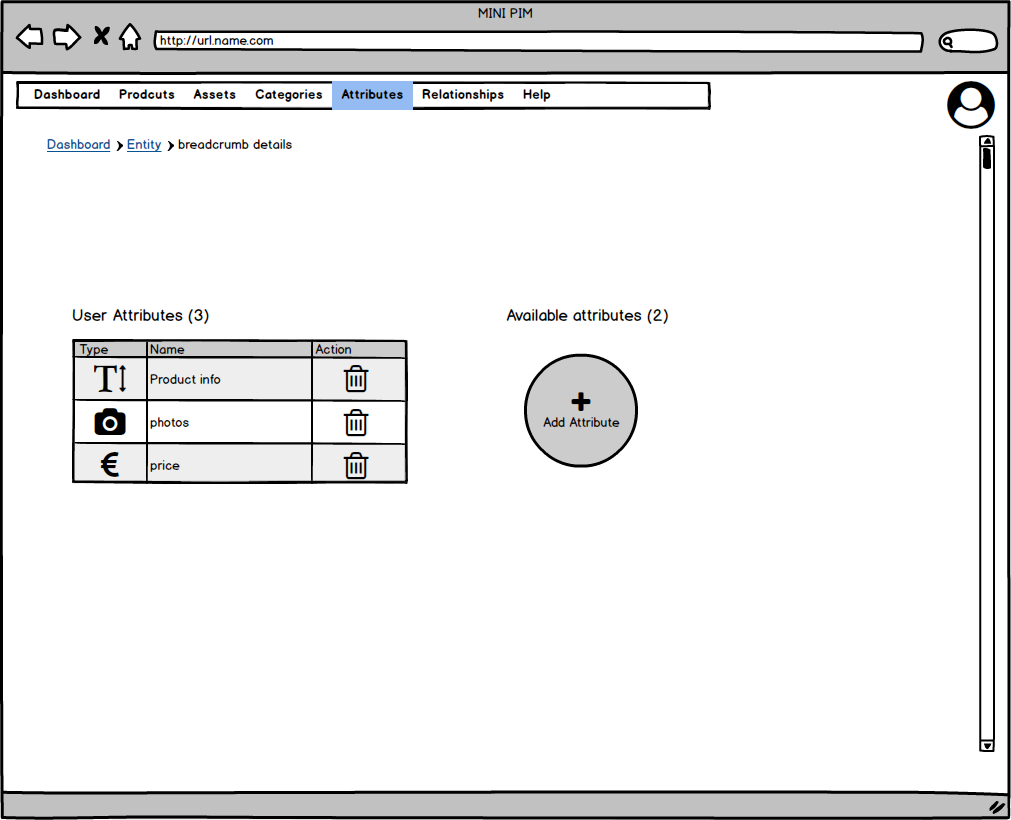
\includegraphics[width=1\linewidth]{mockups/RF6.1Crear_Atributo.png}
    \caption{Apartado Atributos}
   \end{figure}
\vspace{1.0cm}

\newpage %Inicia en una nueva página otro caso de uso